\chapter{Stiff string}\label{ch:stiffString}
Earlier, the case of the ideal string was presented (Section \ref{sec:1DWave}) modelled using the 1D wave equation. As shown, the model generates an output with harmonic partials that are integer multiples of the fundamental frequency. In the real world, however, strings exhibit a phenomenon called \textit{inharmonicity} due to stiffness in the material. 

The restoring force of the 1D wave equation is only due to tension. In the real world, however, this force is also due to stiffness, dependent on the material and geometry of the string. This stiffness causes frequency dispersion and inharmonicity: the partials get exponentially further apart with frequency. 

The stiff string played a prominent part in many of the published works:
\citeP[A], \citeP[B], \citeP[C], \citeP[D] and \citeP[E]. 

This chapter 

\section{Continuous time}
Consider the transverse displacement of a lossless \todo{should I even include the lossless one? It's just so that we can slowly build up to the damped model...}stiff string of length $L$ described by $u=u(x,t)$ defined for $x\in \D$ with domain $\D = [0, L]$ and time $t\geq 0$. The PDE describing its motion is 
\begin{equation}\label{eq:stiffStringPDENoLosses}
    \rho A \ptt u = T \pxx u - EI \pxxxx u
\end{equation}
parameterised by material density $\rho$ (in kg/m$^3$), cross-sectional area $A = \pi r^2$ (in m$^2$), radius $r$ (in m) tension $T$ (in N), Young's modulus $E$ (in Pa) and area moment of inertia $I = \pi r^4/4$ (in m$^4$). If either $E$ or $I$ is 0, Eq \eqref{eq:stiffStringPDENoLosses} reduces to the 1D wave equation in \eqref{eq:1DwavePDE} where $c = \sqrt{T/\rho A}$. If instead $T = 0$, Eq. \eqref{eq:stiffStringPDENoLosses} reduces to the \textit{ideal bar} equation.


\subsubsection{Dispersion Analysis}
The 4th-order spatial derivative models \textit{frequency dispersion}, a phenomenon that causes different frequencies to travel at different speeds. As opposed to the undesired numerical dispersion 

\subsection{Adding Losses}
Before moving on to the discretisation of Eq. \eqref{eq:stiffStringPDENoLosses}, losses can be added to the system. This is done by simply adding terms to \eqref{eq:stiffStringPDENoLosses} according to \todo{First appeared in \cite{Bensa2003}}
\begin{equation}\label{eq:stiffStringPDE}
    \rho A \ptt u = T \pxx u - EI \pxxxx u - 2 \sz \rho A \pt u + 2 \so \rho A\pt \pxx u
\end{equation}
where the loss coefficients $\sz$ (in s$^{-1}$) and $\so$ (in m$^2$/s) describe the frequency dependent and frequency independent losses respectively. 

A more compact way to write Eq. \eqref{eq:stiffStringPDE}, and as is also found often in the literature \cite{theBible} \todo{etc.} is to divide both sides by $\rho A$ to get
\begin{equation}\label{eq:stiffStringPDECompact}
    \ptt u = c^2 \pxx u - \kappa^2 \pxxxx u - 2 \sz \pt u + 2 \so \pt \pxx u
\end{equation}
where $c=\sqrt{T/\rho A}$ is the wave speed \todo{check wavespeed or wave speed (entire document)} (in m/s) as in the 1D wave equation in \eqref{eq:1DwavePDE} and $\kappa = \sqrt{EI / \rho A}$ is a \textit{stiffness coefficient} (in m$^2$/s).

\subsubsection{Intuition}
Although Eq. \eqref{eq:stiffStringPDE} might look daunting at first, the principle of Newton's second law remains the same. 

Something about the 4th spatial derivative and the loss terms here...

\subsubsection{Boundary Conditions}
The boundary conditions found in Eq. \eqref{eq:boundaryCond1DWave} can be extended to
\begin{subequations}\label{eq:stiffStringBoundConds}
    \begin{align}
        u = \px u &= 0 \quad \text{(clamped)}\label{eq:BCclamped}\\
        u = \pxx u &= 0 \quad \text{(simply supported)}\label{eq:BCsimplySupported}\\
        \pxx u = \pxxx u &= 0 \quad \text{(free)}\label{eq:BCfree}
    \end{align}
\end{subequations}
at $x = 0, L$.
\todo{insert figure showing virtual grid points}

\section{Discrete Time}
For the sake of brevity, we continue with Eq. \eqref{eq:stiffStringPDECompact} (rather than Eq. \eqref{eq:stiffStringPDE}) which can be discretised as 
\begin{equation}\label{eq:stiffStringFDS}
    \dtt \uln = c^2 \dxx \uln - \kappa^2 \dxxxx \uln - 2 \sz \dtd \uln + 2 \so\dtm\dxx \uln,
\end{equation}
And domain $l\in\{0, \hdots, N\}$ and number of grid points $N+1$. The stability condition will be derived in Section \ref{sec:stiffStringStability} 

The $\dxxxx$ operator is the second-order spatial difference in Eq. \eqref{eq:discSecondSpace} applied to itself
\begin{equation}\label{eq:dxxxx}
    \dxxxx = \dxx\dxx = \frac{1}{h^4}\left(e_{x+}^2 - 4e_{x+}+6 - 4e_{x-}+e_{x-}^2\right).
\end{equation} \todo{explain the mixed operator here}

The reason a backwards difference is used here is to keep the system explicit. A centred operator could potentially be used, but then neighbouring points at the next time step, i.e., $u^{n+1}_{l+1}$ and $u^{n+1}_{l-1}$ would be needed to calculate $u^{n+1}_l$. 


Using 
\begin{equation}
    \lambda = \frac{ck}{h} \qaq \mu = \frac{\kappa k}{h^2},
\end{equation}
we can expand the operators and collect the terms to obtain the following update equation
\begin{equation}
    \begin{aligned}
    % (1+\sz k) u_l^{n+1} =&\ \left(2 - 2\lambda^2 - 6\mu^2 - \frac{4\so k}{h^2}\right) \uln\\
    % & + \left(\lambda^2 + 4\mu^2 + \frac{2\so k}{h^2}\right) (u_{l+1}^n + u_{l-1}^n) \\
    % &- \mu^2 (u_{l+2}^n + u_{l-2}^n) + \left(-1+\sz k + \frac{4\sz k}{h^2}\right)u_l^{n-1}\\
    % & - \frac{2\so k}{h^2}(u_{l+1}^{n-1} + u_{l-1}^{n-1})
    % \end{aligned}
    Au_l^{n+1} = &\ B_0 \uln + B_1 (u_{l+1}^n + u_{l-1}^n) + B_2 (u_{l+2}^n + u_{l-2}^n) \\
    &+ C_0 u_l^{n-1} + C_1(u_{l+1}^{n-1} + u_{l-1}^{n-1}) 
    \end{aligned}
\end{equation}
with coefficients
\begin{gather*}
    B_0 = 2 - 2\lambda^2 - 6\mu^2 - \frac{4\so k}{h^2}, \quad B_1 = \lambda^2 + 4\mu^2 + \frac{2\so k}{h^2}, \quad B_2 =- \mu^2, \\[1em]
    C_0 =  -1+\sz k + \frac{4\so k}{h^2},\quad C_1 = - \frac{2\so k}{h^2}, \qaq A = 1+\sz k.
\end{gather*}
Note that the division by $A$ has been left for implementation. 
\begin{figure}[h]
    \centering
    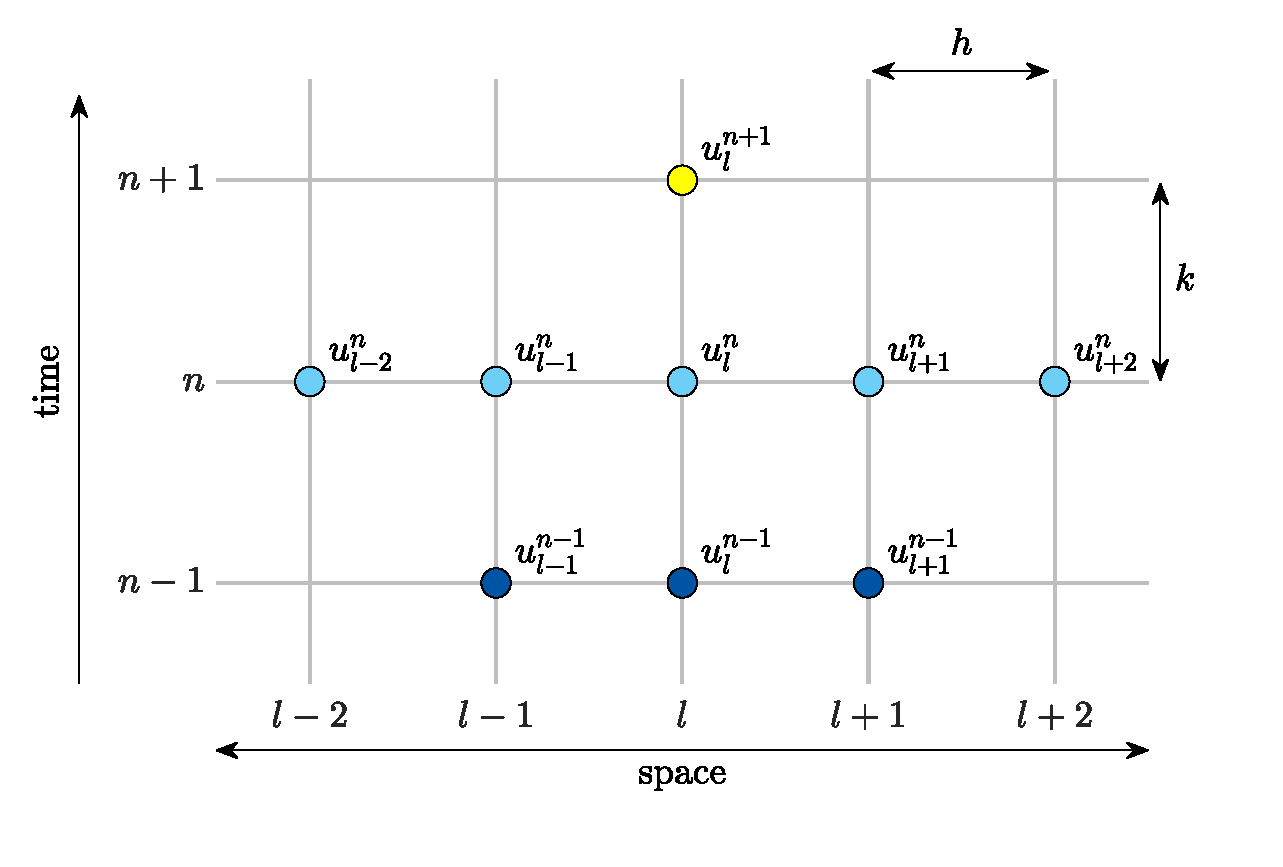
\includegraphics[width=0.8\textwidth]{figures/resonators/stencilDampedStiffString.eps}
    \caption{The stencil for the damped stiff string scheme in \eqref{eq:stiffStringFDS}.\label{fig:stencilStiffString}}
\end{figure}

\subsection{Stability condition}\label{sec:stiffStringStability}
Following the same steps as in 

The stability condition can be shown to be 
\begin{equation}
    h \geq \sqrt{\frac{c^2k^2+4\so k + \sqrt{(c^2k^2 + 4\so k)^2+16\kappa^2k^2}}{2}}
\end{equation}

\subsection{Boundary conditions}
Due to the fourth-order spatial derivative, two virtual grid points need to be accounted for at the boundaries of the system. Discretising the boundary conditions in \eqref{eq:stiffStringBoundConds} yields
\begin{subequations}\label{eq:stiffStringBoundCondsDisc}
    \begin{align}
        \uln = \delta_{x\pm} \uln &= 0 \quad \text{(clamped)}\label{eq:BCclampedDisc}\\
        \uln = \dxx \uln &= 0 \quad \text{(simply supported)}\label{eq:BCsimplySupportedDisc}\\
        \dxx \uln = \dxd\dxx \uln &= 0 \quad \text{(free)}\label{eq:BCfreeDisc}
    \end{align}
\end{subequations}
at $l = 0, L$. The operator in the clamped condition is $\dxp$ at $l = 0$ and $\dxm$ at $l = N$. Expanding these operators for the clamped condition yields 
\begin{equation}
    u_0^n = u_1^n = 0 \qaq u_{N-1}^n = u_N^n = 0.
\end{equation}
This can be simplified by reducing the range of calculation to $l\in \{ 2, \hdots, N-2\}$.

As the end points of a system with simply supported boundary conditions are $0$ at all times, the range of calculation can be reduced to $l\in \{ 1, \hdots, N-1\}$. At $l=1$ and $l=N-1$ the virtual grid points $u_{-1}^n$ and $u_{N+1}^n$ are needed. A definition for $u_{-1}^n$ can be found by expanding Eq. \eqref{eq:BCsimplySupportedDisc} at $l = 0$:
\begin{align}
    &\frac{1}{h^2}\left(u_1^n - 2 u_0^n + u_{-1}^n\right) = 0\nonumber\\[-1em]
    \xLeftrightarrow{\mystrut\ u^n_0 = 0\ } \quad & u_1^n + u_{-1}^n = 0\nonumber\\[0.25em]
    &u_{-1}^n = -u_1^n,\label{eq:simplySupportedResult}
\end{align}
and similarly for $u_{N+1}^n$ by expanding the condition at $l=N$
\begin{equation*}
    u_{N+1}^n = -u_{N-1}^n.
\end{equation*}
The update equations for $l=1$ then becomes
\begin{equation}
    Au_1^{n+1} = B_0 u_1^n + B_1 u_2^n + B_2 (u_3^n - u_1^n) + C_0 u_1^{n-1} + C_1(u_2^{n-1} 
\end{equation}
and for $l=N-1$
\begin{equation}
    Au_{N-1}^{n+1} = B_0 u_{N-1}^n + B_1 u_{N-2}^n + B_2 (u_{N-3}^n - u_{N-1}^n) + C_0 u_{N-1}^{n-1} + C_1(u_{N-2}^{n-1}
\end{equation}

Finally, the free boundary condition requires all points to be calculated and $l\in\{0, \hdots, N\}$. 

The combined operator in Eq. \eqref{eq:BCfreeDisc} is defined as:
\begin{align}
    \dxd\dxx &= \frac{1}{2h^3}\left(e_{x+}-e_{x-}\right)\left(e_{x+}-2+e_{x-}\right),\nonumber\\
    &=\frac{1}{2h^3}\left(e_{x+}^2 - 2e_{x+} + 1 - (1 - 2e_{x-} + e_{x-}^2\right),\nonumber\\
    &=\frac{1}{2h^3}\left(e_{x+}^2 - 2e_{x+} + 2e_{x-} -e_{x-}^2\right).
\end{align}
This can be used to solve for the virtual grid points in the free condition at $l=0$:

\begin{align*}
    \frac{1}{2h^3} &\left(u_2^n - 2 u_1^n + u_{-1}^n - u_{-2}^n\right) = 0\\
    u_{-2}^n &= u_2^n - 2 u_1^n + u_{-1}^n\\
    \xLeftrightarrow{\mystrut\ \dxx \uln = 0\ \Rightarrow\ \text{ Eq. \eqref{eq:simplySupportedResult}}\ }
    \quad u_{-2}^n &= u_2^n - 3 u_1^n 
\end{align*}

\subsection{Combining operators}\label{sec:combiningOperators}
Operators can be combined by simply multiplying their definitions. Recalling the definitions for $\dtm$ in Eq. \eqref{eq:backwardTimeOperator} and $\dxx$ Eq. \eqref{eq:discSecondSpace} their combination results in
\begin{align*}
    \dtm\dxx &= \frac{1}{k}\left(1-e_{t-}\right)\frac{1}{h^2}\left(e_{x+}-2+e_{x-}\right), \\
    &= \frac{1}{kh^2}\left(e_{x+}-2+e_{x-} - e_{t-}(e_{x+}-2+e_{x-})\right).
\end{align*}
%
% Taking the mixed derivative for the 
% \begin{equation*}
%         \dtm \dxx \uln =
%         \begin{cases}
%             \frac{1}{k}\left(\dxx \uln - \dxx u_l^{n-1}\right) & \text{expanding}\ \dtm\\
%             \frac{1}{h^2}\left(\dtm u_{l+1}^n - 2\dtm \uln + \dtm u_{l-1}^n\right) & \text{expanding}\ \dxx
%         \end{cases}
% \end{equation*}
% and after expansion of the second operator both result in
A multiplication of two (different) shift operators applied to a grid function simply means to apply each shift individually. The $\dtm\dxx$ operator applied to $\uln$ thus yields
\begin{equation}
    \dtm \dxx \uln = \frac{1}{hk^2}\left(u_{l+1}^n - 2 \uln + u_{l-1}^n - u_{l+1}^{n-1} + 2 u_l^{n-1} - u_{l-1}^{n-1}\right).
\end{equation}



\section{Modal analysis}
To perform a modal analysis on the FD scheme of the damped stiff string in \eqref{eq:stiffStringFDS} 

The matrix form of the $\dxxxx$ operator in \eqref{eq:dxxxx} with simply supported boundary conditions can be obtained by multiplying two $\Dxx$ matrices according to
\begin{equation}
    \Dxx\Dxx = \mathbf{D}_{xxxx} = \frac{1}{h^4}\begin{bmatrix}
        5& -4 & 1 & & & \mathbf{0}& \\
        -4 & 6 &\ddots &\ddots & & & \\
        1& \ddots & \ddots & -4 & 1 & & \\
        & \ddots& -4 & 6 & -4 & \ddots& \\
        & & 1 & -4 & \ddots & \ddots &1 \\
        & & & \ddots & \ddots & 6 & -4 \\
        & \mathbf{0} & & & 1& -4 & 5 \\
    \end{bmatrix}.
\end{equation}
